\documentclass[a4paper, 12pt, twoside]{book}
\usepackage[activate={true,nocompatibility},
final,
tracking=true,
kerning=true,
spacing=true,
factor=1100,
stretch=10,
shrink=10]{microtype}
\microtypecontext{spacing=nonfrench}

\usepackage{lmodern}
\usepackage[T1]{fontenc}
\usepackage[utf8]{inputenc}
\usepackage[english]{babel}

\usepackage[a4paper, top=2.5cm, bottom=2.5cm, inner=3.0cm, outer=2.5cm, headheight=15pt]{geometry}
\usepackage{parskip} 

\usepackage{amsmath, amssymb, amsthm, bm}


\usepackage{array} % for '\newcolumntype' macro
\newcolumntype{C}{>{{}}c<{{}}} % for binary and relational operators
\newcolumntype{L}{>{\displaystyle}l} % automatic display-style math mode, left-aligned

\theoremstyle{definition}
\newtheorem{theorem}{Theorem}
\newtheorem{definition}[theorem]{Definition}

% \usepackage{titlesec}
% \titleformat{\section}
%   {\normalfont\fontsize{14}{15}\bfseries}
%   {\thesection}{1cm}{}

% \titleformat{\subsection}
%   {\normalfont\fontsize{14}{15}\bfseries}
%   {\thesubsection}{1cm}{}

\usepackage{svg}  
\usepackage{graphicx}
\usepackage{transparent}
\usepackage{eso-pic}

\usepackage[noend]{algorithmic}
\usepackage{algorithm}

\renewcommand{\algorithmicrequire}{\textbf{Input:}}
\renewcommand{\algorithmicensure}{\textbf{Output:}}
\renewcommand{\algorithmicforall}{\textbf{for each}}
\renewcommand{\algorithmiccomment}[1]{// #1}

\usepackage{caption}
\captionsetup{width=0.8\textwidth}
\usepackage{subcaption}

\usepackage[
backend=biber,
style=alphabetic,
sorting=ynt
]{biblatex}
\addbibresource{references.bib}

\usepackage{csquotes}

\usepackage[colorlinks, linkcolor=black, citecolor=black]{hyperref}
\usepackage{url}

\usepackage{fancyhdr}

\pagestyle{fancy}
\fancyhf{}
\fancyhead[LE]{\nouppercase\leftmark}
\fancyhead[RO]{Section \nouppercase\rightmark}
\fancyhead[RE,LO]{\thepage}
\fancyfoot[C]{}

\usepackage{booktabs}

\newcommand{\RomanNumeralCaps}[1]{\MakeUppercase{\romannumeral #1}}





\begin{document}


\frontmatter
 
    \documentclass[../main.tex]{subfiles}
\begin{document}
    
\newcommand\BackgroundPic{%
\put(0,-170){%
\parbox[b][\paperheight]{\paperwidth}{%
\vfill
\centering
{\transparent{0.05} \includesvg[width=0.3\paperwidth,height=0.3\paperheight,%
keepaspectratio]{img/logo.svg}}%
\vfill
}}}


\begin{titlepage}
    \begin{center}
        \vspace*{1cm}
            
        \Huge
        Generative Pattern Dissemination \\
        for Collaborative Intrusion Detection
            
        \vspace{0.5cm}
        \large
            
        \vspace{3cm}
            
            
        \normalsize
        A thesis presented for the degree of Master of Science \\
        by Mike Petersen
        
        \vspace{1.5cm}
        
        First Reviewer: Prof. Dr. Ulrich Bühler \\
        Second Reviewer: Prof. Dr. Sebastian Rieger
            
        \vfill
        % \AddToShipoutPicture*{\BackgroundPic}
            
        \normalsize
        Department of Computer Sciences\\
        University of Applied Sciences Fulda\\
        Fulda, Germany\\
        July 2021
            
    \end{center}
\end{titlepage}

\end{document}
%
    % Preface
    % \documentclass[../main.tex]{subfiles}
\begin{document}

\begingroup

%However, when considering the development of the current threat environment, the effectiveness of conventional intrusion detection systems is limited. Technology trends, such as the internet of things or cloud computing, are main drivers for increasingly blurring corporate boundaries in the context of interconnection of infrastructures and shared resources. This transformation increases the potential attack surface of productive computer systems for large-scale and high-velocity cyber attacks, which traditional IDSs have limited effectiveness due to their isolated nature. For example, such stand-alone IDS will not be able to create connections between security events that occur at different infrastructures simultaneously. Due to the mentioned increase of attack surface that is related to the size of current computer networks, attackers may attempt to obfuscate the characteristic overall sequence of the intrusion by spreading single attack steps.
\hspace{0pt}
\vfill
\begin{adjustwidth}{2cm}{2cm}
\begin{center}
    \small\textbf{Abstract}
\end{center}
\par\medskip

The continuous blurring of corporate boundaries induced by the development of globally networked supply chains and the associated interconnection of IT infrastructures is increasing the potential attack surface and velocity of cyber attacks, which requires the development of innovative defense solutions.
\glspl{cids} attempt to improve attack detection with intelligent mechanisms for information sharing and correlation.
All approaches that implement data dissemination in \gls{cids} face the same key challenges.
On the one hand, privacy must be ensured when exchanging sensitive data, while on the other hand the quality of the data must not be compromised. 
Additionally, the exchange itself may increase the latency of attack detection and thus degrade the overall performance in practice.
In this context, we present a novel \gls{cids} that exchanges generative machine learning models, which resemble original data. 
Specifically, data sets are partitioned using \gls{lsh} and persisted locally in a key-value store by using a corresponding hash value (region) as a component for the key creation.
%TODO: upstream oder downstream?
This way, updates on specific regions are propagated automatically downstream through the processing pipeline, where regions are classified on a global level as either complex or simple with respect to the number of classes they contain.
Complex regions are subject to the generative model selection process, where the respective data in a region is used for the training of a \gls{gmm}, which in turn is shared among members of the \gls{cids} by utilizing the replication capabilities of the key-value store the data is stored in.
By compressing local data into generative models, the exchanged data volume is reduced, like-wise supporting data privacy.
Processing latency is shortened by exploiting parallelization induced by the data partitioning.
By exchanging only hashed values and class labels, data privacy is preserved. 
Multiclass classification experiments on multiple network intrusion datasets demonstrate a superior performance of this approach in comparison to local detection schemes.
\end{adjustwidth}
\vfill
\hspace{0pt}
\par\endgroup
\bigskip\noindent
\end{document}
    % \include{dedication.tex}
    % \include{formal_declaration.tex}
    \tableofcontents%
    \newacronym{ids}{IDS}{Intrusion Detection System}

\newacronym{cids}{CIDS}{Collaborative Intrusion Detection System}

\newacronym{qos}{QoS}{Quality of Service}

\newacronym{pca}{PCA}{Principal Component Analysis}

\newacronym{gmm}{GMM}{Gaussian Mixture Model}

\newacronym{dos}{DoS}{Denial of Service}

\newacronym{r2l}{R2L}{Remote to Local}

\newacronym{u2r}{U2R}{User to Root}

\newacronym{hids}{HIDS}{Host-based Intrusion Detection System}

\newacronym{nids}{NIDS}{Network-based Intrusion Detection System}

\newacronym{dpi}{DPI}{Deep Packet Inspection}

\newacronym{gan}{GAN}{Generative Adversarial Network}

\newacronym{dgm}{DGM}{Deep Generative Models}

\newacronym{lvm}{LVM}{Latent Variable Model}

\newacronym{ema}{EM Algorithm}{Expectation Maximization Algorithm}

\newacronym{mle}{MLE}{Maximum Likelihood Estimation}

\newacronym{onb}{ONB}{Orthonormal Basis}

\newacronym{dr}{DR}{Detection Rate}

\newacronym{fpr}{FPR}{False Postive Rate}

\newacronym{fpf}{FPF}{Flow Processing Format}

\newacronym{cidsm}{CIDSM}{Collaborative Intrusion Detection System Message}

\newacronym{pii}{PII}{Personally Identifiable Information }

\printglossary[type=\acronymtype, title=List of Abbreviations, toctitle=List of Abbreviations]


\mainmatter

    % include an explaination that differentiates between alert data and training data in the ids context (needed for describing the difference to related work)

    \chapter{Introduction}

\section{Motivation}
\input{2_mainmatter/1_introduction/1_motivation.tex}

\section{Objectives}
\input{2_mainmatter/1_introduction/2_objectives.tex}

\section{Structure}
\input{2_mainmatter/1_introduction/3_structure.tex}

% Beschreibung der gestellten Aufgabe
% Rahmenbedingungen
% Einschränkungen
% Vorgaben
% angestrebte Ziele% ~5 pages

    \chapter{Preliminaries}

% Darstellung der theoretischen Grundlagen
% Definition der verwendeten Begriffe
% allgemeine Konzepte und Ansätze

\section{Intrusion Detection}

Classic security mechanisms, such as encryption or firewalls, are considered as preventive measures for protecting IT infrastructures. However, in order to be able to react to security breaches that have already occurred, additional reactive mechanisms are required. To complement preventive measures, Intrusion Detection Systems (IDSs) have been commercially available since the late 1990s \cite[27]{whitman_principles_2018}.

First, IDSs are described and categorized. In the context of the shortcomings of conventional IDSs for protecting large scale systems, Collaborative Intrusion Detection Systems (CIDSs) are introduced.

\subsection{Intrusion Detection Systems}
Generally, the main reason for operating an IDS is to monitor and analyze computer networks or systems in order to identify anomalies, intrusions or privacy violations \cite{hindy2020taxonomy}. Specifically, the following three advantages are significant \cite[391]{whitman_principles_2018}.

\begin{itemize}
    \item IDSs can detect the preliminaries of attacks, in particular the organized gathering of information about networks and defense mechanisms (attack reconnaissance), and thus enable the prevention or mitigation of damage to information assets.
    \item IDSs can help protect information assets when known vulnerabilities cannot be fixed fast enough, notably in the context of an rapidly changing threat environment.
    \item The occurrence of unknown security vulnerabilities (zero day vulnerabilities) is not predictable, meaning that no specific preparations can be made for them. However, IDSs can identify processes in the IT system that deviate from the normal state and thus contribute to the detection of zero day attacks
\end{itemize}

For an effective IDS, it is important to be able to detect as many steps as possible within the typical attack sequence, also called kill chain \cite[393]{whitman_principles_2018}. Since a successful intrusion into a system can be stopped at several points in this sequence, the effectiveness of the IDS increases with its functionality. The following categorization of intrusion attempts according to \cite{kendall1999database} reflects parts of the kill chain mentioned above:

\begin{description}
    \item[Probing] Probing refers to the preambles of actual attacks, also known as attack reconnaissance. This includes obtaining information about an organization and its network behavior (footprinting) and obtaining detailed information about the used operating systems, network protocols or hardware devices (fingerprinting).
    \item[Denial of Service (DoS)] DoS refers to an attack aimed at disabling a particular service for legitimate users by overloading the target systems processing capacity.
    \item[Remote to Local (R2L)] R2L attacks attempt to gain local access to the target system via a network connection.
    \item[User to Root (U2R)] One step further, U2R attacks start out with user access on the system and gain root access by exploiting vulnerabilities.
\end{description}

Additionally, IDS are generally categorized by the platform being monitored and the employed attack detection method \cite{milenkoski2015evaluating}. Hence, a distinction is made between Host-based Intrusion Detection System (HIDS) and Network-based Intrusion Detection System (NIDS). While a HIDS resides on a system, known as host, only monitoring local activities, a NIDS resides on a network segment and monitors remote attacks that are carried out across the segment. Furthermore, IDS are categorized into signature-based detection and anomaly-based detection. A signature-based IDS (also called knowledge-based detection) compares the system or network state against a collection of signatures of known attacks. The false positive rate is very low when using signatures, but only when assuming the system is confronted with already known attacks. Typically, this method cannot detect novel \cite[403]{whitman_principles_2018}, metamorphic or polymorphic attacks \cite[236]{szor2005art}. An anomaly-based IDS, on the other hand, creates a statistical baseline profile of the system’s or network’s regular state and compares it with the monitored activities. This allows both known and unknown attacks to be detected, but the frequent occurrence of false-positive estimations is a major challenge. Furthermore, hybrid models of the presented approaches from the respective categories exist.

\subsection{Flow Capturing and Network Monitoring}

\subsection{Coordinated Attacks}

\subsection{Collaborative Intrusion Detection Systems}

However, when considering the development of the current threat environment, the effectiveness of conventional intrusion detection systems is limited. Technology trends, such as the internet of things or cloud computing, are main drivers for increasingly blurring corporate boundaries in the context of interconnection of infrastructures and shared resources. This transformation increases the potential attack surface of productive computer systems for large-scale and high-velocity cyber attacks, which traditional IDSs have limited effectiveness due to their isolated nature. For example, such stand-alone IDS will not be able to create connections between security events that occur at different infrastructures simultaneously. Due to the mentioned increase of attack surface that is related to the size of current computer networks, attackers may attempt to obfuscate the characteristic overall sequence of the intrusion by spreading single attack steps.

n order to address the aforementioned security problems of large IT systems, Collaborative Intrusion Detection Systems (CIDSs) have been proposed. In general, a CIDS is a network of several intrusion detection components that collect and exchange data on system security. A CIDS is essentially specified by two different types of components, namely the detection units and the correlation units, and their communication among each other. The detections units can be considered as conventional IDS that monitor a sub-network or a host and by that, generate low-level intrusion alerts. The correlation unit is responsible for merging the low-level intrusion alerts and their further post-processing. This includes, for instance, the correlation of the alerts, the generation of reports or the distribution of the information to the participants of the network. CIDSs pursue the following two goals \cite[24]{vasilomanolakis_collaborative_2016}.

\begin{itemize}
    \item The aggregation and correlation of data originating from different IDSs creates a holistic picture of the network to be monitored and enables the detection of distributed and coordinated attacks.
    \item CIDSs can monitor large-scale networks more effectively with the realization of a loadbalancing strategy. By sharing IDS resources across different infrastructures, short-term peak loads can be served, reducing the downtime of individual IDSs.
\end{itemize}



\section{Gaussian Mixture Models}

\subsection{Gaussian Distribution}

\subsection{Density Estimation}

\subsection{Gaussian Mixtures}



\newpage
\section{Locality Sensitive Hashing}
Finding similar objects, formally known as the nearest-neighbour search problem, is a central problem in computer science in general. And besides the exact search, it is also an important topic in the field of intrusion detection. For example, exact searches allow to compare the signatures of known malware with low false positive rates. Considering polymorphic attacks, however, it is essential to also detect all objects that are similar to the known attack and thus detect modified forms of it. In this context, this section presents a well-studied approach called \textit{Locality Sensitive Hashing} (LSH) that solves an approximate version of the nearest-neighbour search problem by partitioning the search space with a hash function. This way, the searching problem is reduced to pairs that are most likely to be similar. Besides the application for solving the NN search problem, for which LSH was originally conceived, the concept has been proven to be effective for numerous other use cases, such as dimensionality reduction, clustering or classification. As the proposed generative pattern database integrates a locality-sensitive hash function for enabling both similarity search and data parallelism, LSH and a specific variant called \textit{Random Projection} (RP) is described in detail in this section.

Section \ref{subsec:approximate_nearest_neighbour_problem} introduces the approximate version of the nearest neighbour search problem as it is a prerequisite for the general definition of LSH. After that, Section \ref{subsec:locality-sensitive-hashes} begins by clarifying the core idea of LSH and subsequently explains how to construct a locality-sensitive hash function. Lastly, a specific family of LSH that uses the cosine distance for similarity calculations, also known as \textit{Random Projection} is presented in Section \ref{subsec:random_projection}.

\subsection{The Approximate Nearest Neigbour Problem}\label{subsec:approximate_nearest_neighbour_problem}

For all definitions of the NN and its variants, a set of $n$ points $P = \{p_1, \dots, p_n \}$ in a metric space $(X, d)$ where $P \subset X$ is considered.\footnote{It is assumed that $d$ is a proper \textit{metric}, which means that it is \textit{symmetric}: $d(p,q)=d(q,p)$ , \textit{reflexive}: $d(p,q) \leq 0$, $d(p,q)=0 \iff p=q$ and satisfies the \textit{triangle inequality}: $d(p,q) \leq d(p,s) + d(s,q)$.} Then, the general NN is stated as follows.

\begin{definition}[Nearest Neigbour Problem]\label{def:nn}
     Construct a data structure so as to efficiently answer the following query: Given any query point $q$, find some point $p \in P$ such that
    \begin{equation}
        \mathop{\text{min}}_{q \in X} \; d(p, q).
    \end{equation}
\end{definition}

A specific example of Definition \ref{def:nn} could include high-dimensional data in $P \in \mathbb{R}^k$ with $k \gg 1$ and define $d$ as the euclidean distance. In this case, an exhaustive search would require a query time of $O(kn)$. Unfortunately, all exact algorithms that provide a better time complexity than an exhaustive search require $O(2^k)$ space \cite{rubinstein2018hardness}. This tradeoff between time and space complexity is usually referred to as ``curse of dimensionality'' and can only be resolved by accepting approximate solutions. The $c$-approximate nearest neighbour problem ($c$-ANN) is defined as follows.

\begin{definition}[$c$-Approximate Nearest Neighbour Problem]
    For any given query point $q \in X$ and some approximation factor $c > 1$, find some point $p \in P$ such that
    \begin{equation}
        d(q,p) < c \cdot \mathop{\text{min}}_{s \in P} \; d(s, q).
    \end{equation}
\end{definition}

Thus, the distance from the query point $q$ to the approximate nearest neighbour $p$ is at most $c$ times the distance to the true nearest neighbour $s$. Strictly speaking, LSH does not solve the $c$-ANN directly. Instead, Indyk and Motwani relaxed the problem by introducing the $cR$-approximate nearest neighbour problem ($cR$-ANN) as follows.

\begin{definition}[$cR$-Approximate Nearest Neighbour Problem]
    For any given query point $q \in X$, some approximation factor $c > 1$ and some target distance $R > 0$, if there exists a point $p \in P$ where $d(p,q) \leq R$, then return a point $p' \in P$ where
    \begin{equation}
        d(p',q) \leq cR.
    \end{equation}
\end{definition}

Figure \ref{fig:nearest_neighbour} illustrates  the $cR$-ANN. The target distance $R$ represents the distance of the query object from its nearest neighbour. If there is such a point, the algorithm returns points within $cR$ distance from the query object. Otherwise it returns nothing. It is shown that LSH can solve the $c$-ANN by solving the $cR$-ANN for different settings of $R$ \cite{indyk_approximate_1998}.

\begin{figure}[t!]
    \centering
    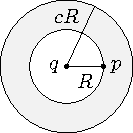
\includegraphics[width=0.3\linewidth]{tikz/nearest_neighbour.pdf}
    \caption{In the $cR$-approximate nearest neighbour problem some point within $cR$ is accepted, if there exists a point $p$ where $d(p,q) \leq R$.}
    \label{fig:nearest_neighbour}
\end{figure}

\subsection{Locality-Sensitive Hash Functions} \label{subsec:locality-sensitive-hashes}

Introduced by Indyck and Motwani in 1998 \cite{indyk_approximate_1998} as an algorithm that solves the approximate nearest neighbour problem (ANN), locality-sensitive hashing (LSH) has since been extensively researched and is now considered among the state of the art for approximate searches in high-dimensional spaces.\footnote{See \cite{nagarkar2021exploring} for an exhaustive survey of NN-Search Techniques.} The basic idea of the approach is to partition the input data using a hash function that is sensitive to the location of the input within the metric space. This way, similar inputs collide with a higher probability than inputs that are far apart. Thus, LSH exhibits fundamental differences to conventional hash functions \footnote{In the following, cryptographic and non-cryptograhpic hash functions are referred to as conventional hashing.}, although the most general definition applies to both.

A hash function is a function that maps a large input set to a smaller target set. The elements of the input set are called \textit{messages} or \textit{keys} and may be of arbitrary different lengths. The elements of the target set are called \textit{digests} or \textit{hash values} and are of fixed size length.

More specifically, we define a hash function as $h: A \rightarrow B : \bm{p} \mapsto \bm{u}$ where $A \subset \mathbb{R}^d$ with $d \in \mathbb{N}$ is the input set and $B=\{0, 1\}^k$ with $k \in \mathbb{N}$ the target set of all bit sequences of fixed size $k$, with $k < d$. According to the notation in \cite[256]{cormen2022introduction}, a hash table is defined by a hash function $h$, that maps the keyspace $K$ into the slots of a hash table $T[0 \,.\,.\, S-1], S \in \mathbb{N}$, i.e. $h: K \rightarrow \{0, 1, \dots, S-1\}$ with $S \ll |K|$. Thus, a message with key $k \in K$ hashes to slot $h(k)$. Additionally, $h(k)$ is the hash value of the key $k$.


% 1. Give formal definitions of Hash function and Hash table
% 2. Explain the difference of conventional hash function and LSH
% 3. Explain the big picture of the algorithm
%%%%%%%%%%%%%%%%%%%%%%%%%%%%%%%%%%%%%%


Typically, conventional hashing is used for the realization of, e.g. hash tables, data integrity checks, error correction methods or database indexes. Depending on the application, different requirements are imposed on the utilized hash function. In this context, the most important property of a hash function is the probability of a \textit{collision}. A collision occurs when two keys $\bm{p}_1 \neq \bm{p}_2$ are projected onto the same hash value $\bm{u} = h(\bm{p}_1) = h(\bm{p}_2)$. For example, cryptographic hash functions are used in systems, where adversaries try to break such systems. Thus, different security requirements are defined for cryptograhpic hash functions \cite[349]{williamcryptography}. In particular, these hash functions are designed to be resistant against collisions, which is the key difference to LSH. Applications that do not require the hash function to be resistant against adversaries, e.g. hash tables, caches or de-duplication, are usually implemented by using a hash function that exhibits relaxed guarantees on the security properties in exchange for significant performance improvements. However, locality-sensitive hashes behave differently as illustrated in Figure \ref{fig:hashing_differences}. LSH projects similar inputs onto the same or near elements. In contrast, conventional hashing tries to distribute projections onto the elements of the target as randomly as possible.

\begin{figure}[t!]
    \centering
    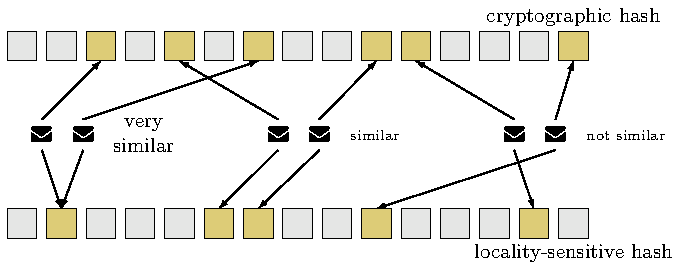
\includegraphics[width=0.8\linewidth]{tikz/hashing_differences.pdf}
    \caption{The behaviour of conventional hashing and LSH}
    \label{fig:hashing_differences}
\end{figure}




%%%%%%%%%%%%%%%%%%%%%%%%%%%%%%%%%%%%%%


% explain the idea of LSH (reduce the search space and then pick a random p or do a linear scan within the reduced search space)

As a locality-sensitive hashing function can be constructed as a general concept, specific families of functions can be derived. We refer to a \textit{family} of hash functions $\mathcal{H}: A \rightarrow B$ as a collection of hash functions that have the same domain and range, share a basic structure and are only differentiated by constants. Three basic requirements are demanded for such a family of functions \cite[99]{leskovec_rajaraman_ullman_2014}.

\begin{enumerate}
    \item Close pairs of input should be hashed in to the same bucket with higher probability than distant pairs.
    \item Specific functions of a family need to be statistically independent, such that the FPR and FNR can be improved by combining two or more functions.
    \item Functions need to be efficient, i.e., be faster compared to an exhaustive search.

\end{enumerate}

The first step is to define LSH generally. Applied on the $cR$-ANN, the first requirement states, with high probability, two points $p$ and $q$ should hash to the same hash value if their distance is at most $R$, i.e., $d(p,q) \leq R$. And if their distance is at least $cR$, the points should hash to different hash values, i.e. $d(p,q) > cR$. Thus,  A formal definition of a locality-sensitive hash function is given as follows \cite{andoni2006near}.

\begin{definition}[Locality-Sesitive Hash Function]
    Given a target distance $R \in \mathbb{R}, R>0$, an approximation factor $c \in \mathbb{R}, c>1$ and probability thresholds $P_1, P_2 \in \mathbb{R}$, a family $\mathcal{H} = \{h: A \rightarrow B$\} is called $(R, cR, P_1, P_2)$-sensitive if for any two points $p,q \in A$ and any hash function $h$ chosen uniformly at random from $\mathcal{H}$ the following conditions are satisfied:
        \[
        \setlength\arraycolsep{0pt}
        \renewcommand\arraystretch{1.2}
            \begin{array}{LCL}
                d(p,q) \leq R & \implies & P[h(p)=h(q)] \geq P_1, \\
                d(p,q) \geq cR & \implies & P[h(p)=h(q)] \leq P_2.
            \end{array}
        \]
\end{definition}
 
Ideally, the gap between $P_1$ and $P_2$ should be as big as possible as depicted in Figure \ref{subfig:exact_probability}, which in fact represents an exact search. This is, as already discussed, no option due to its time and space requirements. Considering a single locality-sensitive function as shown in Figure \ref{subfig:lsh_probability}, where the probability gap between $P_1$ and $P_2$ is relatively close, the false negative rate would be relatively high. Increasing the gap would require to increase $c$ and lead to a high number of false positives. Therefore, a single function would provide only a tradeoff. But it is possible to increase $P_1$ close to $1$ and decrease $P_2$ close to $1/n$ while keeping $R$ and $cR$ fixed as shown in Figure \ref{subfig:lsh_probability_boosted} by introducing a process called \textit{amplification}. Two different forms, namely the AND-construction and the OR-construction, can be applied.

\begin{figure}
    \centering
    \begin{subfigure}[b]{0.3\textwidth}
        \centering
        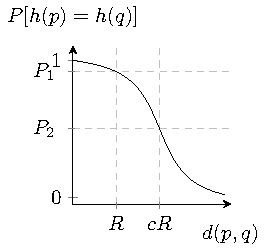
\includegraphics[width=\textwidth]{tikz/lsh_probability.pdf}
        \caption{Single LSH Function.}
        \label{subfig:lsh_probability}
    \end{subfigure}
    \hfill
    \begin{subfigure}[b]{0.3\textwidth}
        \centering
        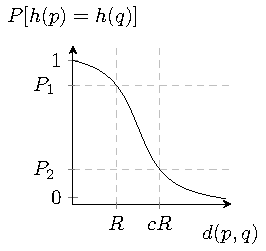
\includegraphics[width=\textwidth]{tikz/lsh_probability_boosted.pdf}
        \caption{Amplified LSH Function.}
        \label{subfig:lsh_probability_boosted}
        \end{subfigure}
        \hfill
        \begin{subfigure}[b]{0.3\textwidth}
            \centering
            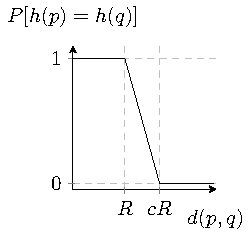
\includegraphics[width=\textwidth]{tikz/exact_probability.pdf}
            \caption{Exact Search}
            \label{subfig:exact_probability}
    \end{subfigure}
    \caption{The behaviour of a $(R, cR, P_1, P_2)$-sensitive function in (\ref{sub@subfig:lsh_probability}) and (\ref{sub@subfig:lsh_probability_boosted}) (adapted from \cite[100]{leskovec_rajaraman_ullman_2014}) approaching the ideal probability gap in (\ref{sub@subfig:exact_probability}) resembling the behaviour of an exact search.}
    \label{fig:lsh_probability}
\end{figure}
   
By applying a logical AND-construction on $\mathcal{H}$ the threshold $P_2$ is reduced. For that, sample $K$ hash functions indepedently from $\mathcal{H}$ and hash each point $p \in P$ to a $K$-dimensional vector with a new constructed function $g \in \mathcal{H}^K$ as

\begin{equation}\label{eq:or_construction}
    g(p) = [h_1(p), h_2(p), \dots, h_K(p)].
\end{equation}

Since all hash functions $\{h_1, \dots, h_K\} \in \mathcal{H}$ are statistically independent the product rule applies and for any two points $p$ and $q$, a collision occurs if and only if $h_i(p)=h_i(q)$ for all $k \in \{1, \dots, K\}$. The probability gap is then defined as follows:

\begin{align}
    P[h_i(p)=h_i(q)] \geq P_1 \implies P[g(p)=g(q)] \geq P_1^K \\
    P[h_i(p)=h_i(q)] \leq P_2 \implies P[g(p)=g(q)] \leq P_2^K.
\end{align}

Thus, by increasing $K$ the threshold $P_2$ can be arbitrarily decreased and approaches zero. However, the AND-construction lowers both $P_1$ and $P_2$. In order to improve $P_1$, the OR-construction is introduced. For that, a number of $L \in \mathbb{N}$ functions $\{g_1, \dots, g_L\}$ are constructed, where each function $g_l, \; l \in \{1, \dots, L\}$ stems from a different family $\mathcal{H}_l$. Note, that the algorithm is successful, when the two points $p, q$ collide at least once for some $g_l$. Therefore, hashing a point $p \in P$ with each $g_l$ results in the following probability for collision.

\begin{align}
    P[\exists l, g_l(p)=g_l(q)] &= 1 - P[\forall l, g_l(p) \neq g_l(q)] \\
                                &= 1 - P[g_l(p) \neq g_l(q)]^L \\
                                &\geq 1 - (1-P_1^K)^L
\end{align}

As the AND-construction lowers both $P_1$ and $P_2$, similarly the OR-construction rises both thresholds. By choosing $K$ and $L$ judiciously, $P_2$ approaches zero while $P_1$ approaches one. Both constructions may be concatenated in any order to manipulate $P_1$ and $P_2$. Of course, the more constructions are used and the higher the values for the parameters $K$ and $L$ are picked, the more time is considered for the application of the function. 

The general algorithm for solving the $cR$-ANN using LSH consists of two consecutive steps. First, a set of points is required for the construction of the data structrue as described in Algorithm \ref{alg:lsh_preprocess}. For each function $g_l$ a corresponding hash table $T_l$ is initialized that will store all data points $p_n$. In other words, all data points are preprocessed and stored $L$ times.The resulting data structure represents the database, which is searched through, when answering a query. Note, that a common collision handling method, such as seperate chaining for example, is applied if a certain slot is already occupied. 

\begin{algorithm}
    \caption{LSH Preprocessing}
    \label{alg:lsh_preprocess}
    \algsetup{indent=2em}
    \begin{algorithmic}[1]
        \REQUIRE $N$ points $p_n \in P$ with $n \in \{1, \dots, N\}, N \in \mathbb{N}$
        \ENSURE data structure $\{T_1, \dots, T_L\}$
        \STATE construct hash functions $g_1, \dots, g_L$ each of length $K$ (see Equation \ref{eq:or_construction})
        \FORALL{$g_l \in \{g_1, \dots, g_L\}$}
            \STATE $T_l \leftarrow$ new HashTable
            \FORALL{$p_n \in P$}
                \STATE add $p_n$ to $T_l[g_l(p_n)]$
            \ENDFOR
        \ENDFOR
    \end{algorithmic}
 \end{algorithm}

 Answering a query point $q$ is done by hashing it multiple times for each $g_l$ as in the preprocessing step (see Algorithm \ref{alg:lsh_query}). Each time, a set of points $P$, stored in the correspoding hash table $T_l$ at the slot $g_l(q)$, are retrieved. That is, identify all $p_n$, such that $g_l(p_n) = g_l(q)$. For each identified $p_n$, a distance function evaluates if the distance $d(p_n, q)$ is within the search perimeter $cR$. If positive, the point is added to the result set $S$, which is returned at the end of the algorithm.

 \begin{algorithm}
    \caption{LSH Query}
    \label{alg:lsh_query}
    \algsetup{indent=2em}
    \begin{algorithmic}[1]
        \REQUIRE a query point $q$ and data structure $\{T_1, \dots, T_L\}$
        \ENSURE a set $S$ of nearest neighours of $q$
        \STATE $S \leftarrow \emptyset$
        \FORALL{$g_l \in \{g_1, \dots, g_L\}$}
            \STATE $P \leftarrow T_l[g_l(q)]$
            \IF{$|P| > 0$}
                \FORALL{$p_n \in P$}
                    \IF{$d(p_n,q) \leq cR$}
                        \STATE add $p_n$ to $S$
                    \ENDIF
                \ENDFOR
            \ENDIF
        \ENDFOR
        \RETURN $S$
    \end{algorithmic}
 \end{algorithm}

 With regard to preprocessing, the consideration of space complexity of Algorithm \ref{alg:lsh_preprocess} is interesting, whereas the runtime of Algorithm \ref{alg:lsh_query} is the most relevant when examining the execution of queries. Fortunately, lower bounds on both quantities have been proven in \cite{motwani2006lower}, resulting in the following theorem.

\begin{theorem}
    Let $(X,d)$ be a metric on a subset of $\mathbb{R}^d$. Given a $(R, cR, P_1, P_2)$-locality sensitive hash family $\mathcal{H}$ and write $\rho = \frac{\text{log}(1/P_1)}{\text{log}(1/P_2)}$. Then for $n = |X|$ and for any $n \geq \frac{1}{P_2}$ there exists a solution to the $cR$-ANN with space complexity $O(dn+n^{1+\rho})$ and query time of $O(n^{\rho})$.
\end{theorem}

Therefore, it follows that the query time of LSH can only be sublinear, if $\rho < 1$, which is the case if the inequality $P_1 > P_2$ is satisfied.



\subsection{Random Projection}\label{subsec:random_projection}

This section presents a specific family $\mathcal{H}$ that is locality-sensitive. The algorithm that bases on this family is known as Gaussian Random Projection (GRP). This approach utilizes the cosine similarity of two real vectors in order to determine their similarity. In the course of this section, basic definitions for Cosine Distance and Cosine Similarity are introduced. Then, the individual calculation steps of the approach are specified. Finally, a visual proof verifies that GRP is a form of LSH.

The cosine distance can be applied in euclidean spaces and discrete versions of euclidean spaces \cite[95]{leskovec_rajaraman_ullman_2014}. For two real vectors $p_1$ and $p_2$, the cosine distance between is equal to the the angle between $p_1$ and $p_2$, regardless of the dimensionality of the space. Note, that by applying the arc-cosine function, the result is in the range $[0, 180]$. The following definition formalizes what has been stated so far.

\begin{definition}[Cosine Distance]
    Given two vectors $p_1$ and $p_2$, the cosine distance $\theta(p_1, p_2)$ is the dot product of $p_1$ and $p_2$ divided by their euclidean distances from the origin ($L_2$-norm):
    \begin{equation}
        \theta(\bm{p}_1, \bm{p}_2) = \text{cos}^{-1} \bigg( \frac{\bm{p}_1 \cdot \bm{p}_2}{||\bm{p}_1|| \: ||\bm{p}_2||} \Bigg).
    \end{equation}
\end{definition}

The angle $\theta$ can be normalized to the range $[0, 1]$ by dividing it by $\pi$. This way, the cosine similarity is simply given by the following definition.

\begin{definition}[Cosine Similarity]
    The cosine similarity is computed as
    \begin{equation}
        1- \frac{\theta(\bm{p}_1, \bm{p}_2)}{\pi}
    \end{equation}
\end{definition}

Introduced in \cite{charikar2002similarity}, the GRP is defined as follows. Given a message $\bm{x} \in A = \{x \in \mathbb{R}^D : 0 \leq x \leq 1 \}$ and a randomly selected hyperplane defined as $\bm{M}=(a_{ij}) \in \mathbb{R}^{D \times K}$ where $a \sim \mathcal{N}(0, I)$, a \textit{gaussian random projection (GRP)} aims to (\RomanNumeralCaps{1}) reduce the dimensionality from $D$ to $L$ dimensions and (\RomanNumeralCaps{2}) provide a binary encoding by first projecting $\bm{x}$ onto $\bm{M}$ and subsequently applying the sign function to each element of the result, which can be formalized as

\begin{gather}
    h(\bm{x}) = [h(\bm{x}, a_1), \dots, h(\bm{x}, a_k)] \text{ with } h(\bm{x}, a) = sign(\bm{x}^Ta) \\
    \text{with } sign(x) = \Biggl\{ \begin{array}{lc}
        0 & \text{if } x < 0, \\
        1 & \text{if } x \geq 0.
    \end{array}
\end{gather}

An illistration of a random hyperplane that dissects the three-dimensional space and partitions the data space is given in Figure \ref{subfig:rp_3d}. The resulting digest $h(x)$ is a binary vector $h(\bm{x}) = \bm{u} \in B = \{0, 1\}^l$ that is used as bucket index for storing $\bm{x}$ in a hash table. For any two messages $\bm{x}_1, \bm{x}_2$, the probability of being hashed to the same bucket increases with a decreasing distance, given as

\begin{equation}\label{eq:rp_proba}
    P[h(\bm{x}_1) = h(\bm{x}_2)] = 1 - \frac{\theta(\bm{x}_1, \bm{x}_2)}{\pi}.
\end{equation}

\begin{figure}[b]
    \centering
    \begin{subfigure}[b]{0.45\textwidth}
        \centering
        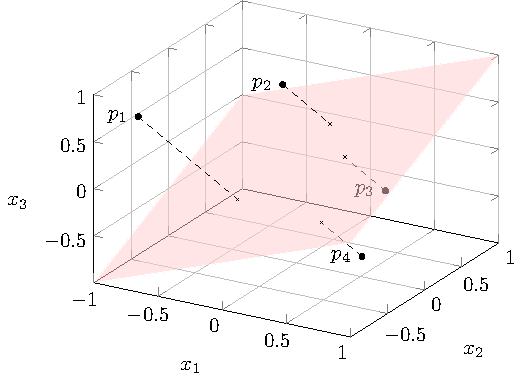
\includegraphics[width=\textwidth]{tikz/random_projection.pdf}
        \caption{Illustration of a random hyperplane (red) partitioning the space.}
        \label{subfig:rp_3d}
    \end{subfigure}
    \hfill
    \begin{subfigure}[b]{0.45\textwidth}
        \centering
        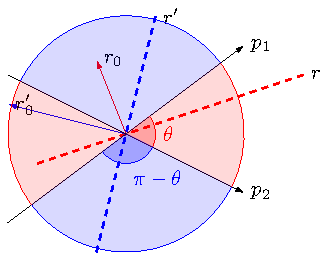
\includegraphics[width=\textwidth]{tikz/random_hyperplane_2d.pdf}
        \caption{Visual Proof of claim in equation \ref{eq:rp_proba}}
        \label{subfig:rp_2d}
    \end{subfigure}
    \caption{}
    \label{fig:random_projection}
\end{figure}

Consider Figure \ref{subfig:rp_2d}, where two vectors $p_1$ and $p_2$, regardless of their dimensionality, define a plane and an angle $\theta$ in this plane.

Pick a hyperplane (actually the normal vector to the hyperplane; hyperplane $v$ is the set of points whose dot product with $v$ is 0)

Hyperplane intersects the plane that is spanned by two vectors $p_1$ and $p_2$ in a line

vector $r_0$ that is normal to the hyperplane represented by the red dashed line; $p_1$ and $p_2$ are on different sides of the hyperplane, thus the projections given by $\langle p_1, r_0 \rangle$ and  $\langle p_2, r_0 \rangle$ will have different signs

vector $r'_0$ that is normal to the hyperplane represented by the blue dashed line;  both $\langle p_1, r'_0 \rangle$ and  $\langle p_2, r'_0 \rangle$ will have the same sign

All angles between the intersection line of the random hyperplane and the plane spanned by $p_1$ and $p_2$ are equally likely. Thus, the probability that the hyperplane looks like the red line is $\theta / \pi$ and like the blue line otherwise.

random projections is a $(R, cR, (1-R/\pi), (1-cR/\pi))$-sensitive family for any $R$ and $cR$. As already explained in Section \ref{subsec:locality-sensitive-hashes}, such a family can be amplified as desired.



% We define a hash function as $h: A \rightarrow B : \bm{p} \mapsto \bm{u}$ where $A \subset \mathbb{R}^d$ with $d \in \mathbb{N}$ is the set of real input data points and $B=\{0, 1\}^l$ with $l \in \mathbb{N}$ the set of all bit sequences of fixed size $l$, with $l < d$. Inputs $\bm{p}$ to hash functions are called \textit{messages} and outputs $\bm{u}$ are called \textit{digests}. 
% A collision occurs when two messages $\bm{p}_1 \neq \bm{p}_2$ are projected onto the same digest $\bm{u} = h(\bm{p}_1) = h(\bm{p}_2)$. We further refer to a \textit{family} of hash functions $\mathcal{H}: A \rightarrow B$ as a collection of hash functions that have the same domain and range, share a basic structure and are only differentiated by constants.

% \subsection{Cryptographic Hash Functions}

% In order to be suitable for cryptographic applications, a hash function $h$ should have, among others, three basic properties. The \textit{first preimage resistance} defines, that for any given $\bm{u} \in B$ it is infeasible to determine any $\bm{p} \in A$ such that $h(\bm{p})=\bm{u}$, allowing $h$ to be effectively one-way only. Furthermore, the \textit{second preimage resistance} defines, that for any given $\bm{p} \in A$ it is infeasible to determine any other $\bm{p}' \in A,\; \bm{p} \neq \bm{p}$ which produces the same output, i.e. $h(\bm{p})=h(\bm{p}')$. Lastly, the \textit{strong collision resistance} states, that is infeasible to determine any two distinct $\bm{p} \neq \bm{p}' \in A$ such that $h(\bm{p})=h(\bm{p}')$.

% \subsection{Non-Cryptographic Hashes} \label{subsubsec:non-cryptographic-hashes}
% Applications that do not require the hash function to be resistant against adversaries, e.g. hash tables, caches or de-duplication, are usually implemented by using a hash function that exhibits relaxed guarantees on the properties defined before in \ref{subsubsec:cryptographic_hashes} in exchange for significant performance improvements.

% \subsection{Locality Sensitive Hash Functions}
% Introduced as an algorithm that solves the $cR$-near neighbour problem, locality-sensitive hashing (LSH) \cite{indyk_approximate_1998} maps similar messages to the same digest with higher probability than dissimilar messages. More formally, given a threshold $R \in \mathbb{R}^{>0}$, an approximation factor $c \in \mathbb{R}^{>1}$ and probabilities $P_1, P_2 \in \mathbb{R}^{\geq 0}$, a family $\mathcal{H}: A \rightarrow B$ is called $(R, cR, P_1, P_2)$-sensitive if for any two points $\bm{p}_1, \bm{p}_2 \in A$ and any hash function $h$ chosen uniformly at random from $\mathcal{H}$ the following conditions are satisfied:

% \begin{itemize}
%     \item if $|| \bm{p}_1 - \bm{p}_2 || \leq R$ then $P[h(\bm{p}_1)=h(\bm{p}_2)] \geq P_1$,
%     \item if $|| \bm{p}_1 - \bm{p}_2 || \geq cR$ then $P[h(\bm{p}_1)=h(\bm{p}_2)] \leq P_2$.
% \end{itemize}

% In order for a $\mathcal{H}$ to be applicable for the $cR$-near neighbour problem, it has to satisfy the inequality $P_1 > P_2$.% ~15 pages

    \chapter{State of the Art}

\section{Data Dissemination in Collaborative Intrusion Detection}

\subsection{Requirements}

\subsection{Centralized and Hierarchical CIDS}

\subsection{Distributed Architectures}

The key components for designing a CIDS architecture are described in \cite[p. 34]{vasilomanolakis_collaborative_2016}. Among them, data dissemination is particularly noteworthy as one of the fundamental components for the communication between members. A central aspect is the communication \textit{overhead} that is introduced with the dissemination of alerts and knowledge within a CIDS, which in turn is heavily influenced by the CIDS architecture \cite[p.39]{vasilomanolakis_collaborative_2016}, that can be primarily categorized into centralized, hierarchical and decentralized approaches \cite{Zhou2010} (see Figure \ref{fig:architectures}). Centralized architectures, consisting of multiple monitoring units and a central analysis unit \cite{Cuppens2002}\cite{Miller2003}, suffer from a Single Point of Failure (SPoF) and are limited in their scalability due to a bottleneck, which is introduced by the central analysis unit. However, the SPoF problem can be mitigated if individual components in such a system are implemented redundantly and form a centralized architecture only at the logical level. A bottleneck, on the other hand, is usually avoided by a distributed implementation, which can also logically be regarded as a central data repository. Hierarchical designs exhibit multiple monitoring and analysis units organized in a tree-based topology \cite{Phillip1997,Zhang2001,Nguyen2019}. These systems are restricted in their scalability by the respective instances on higher levels, whose failure results in a malfunction of the respective sub-trees \cite{Zhou2010}. Again, such disadvantages only play a major role in non-redundantly implemented systems. Additionally, there exist approaches that are inherently distributed. Distributed architectures \cite{Vasilomanolakis2015SkipMon,Perez2013,Bye2008,Fung2008,Janakiraman2003}, wherein each participating system has a monitoring and analysis feature and where the communication is based on some form of data distribution protocol, are considered as scalable by design. However, they depend on effective and consistent data dissemination and the data attribute selected for correlation may affect load distribution among participants~\cite{Zhou2010}.

% \begin{figure}[ht]
%     \centering
%     \includegraphics[width=0.75\textwidth, trim = 1cm 3cm 1cm 5cm ,clip]{img/architectures.pdf}
%     \caption{Overview of centralized (a), hierarchical (b) and distributed (c) CIDS architectures that consist of monitoring units (M) and analysis units (A) or a combination of both (MA).}
%     \label{fig:architectures}
% \end{figure}

The flow of information in centralized and hierarchical architectures is governed by the logical arrangement of components and their specific role. In centralized architectures, there is usually a central entity that controls communication. In hierarchical systems, the communication paths are mainly governed by the topological structure. In contrast to that, different techniques exist in distributed approaches. Whereas flooding refers to unfiltered data distribution to all members, selective techniques reduce the overhead by using, e.g., random walks \cite{Vishnumurthy2006}, gossipping approaches \cite{Dash2006}\cite{Ganesh2003} or publish-subscribe mechanisms. The latter provide flexible organization options and guarantee delivery. For example, subscriptions utilized in \cite{Janakiraman2003} are based on special attack forms.

The data dissemination strategy of a CIDS not only defines the communication paths as described above, but also influences what kind of data is exchanged between the CIDS members while also specifying format and level of granularity. This also includes the central aspects of \textit{data privacy}, realized by utilization of, e.g., bloom filters \cite{Vasilomanolakis2015SkipMon}\cite{Locasto2005}, and \textit{interoperability} that can be obtained by standardized formats, such as the Intrusion Detection Message Exchange Format \cite{Cuppens2002}\cite{Duma2006}.

In particular, there are two approaches to mention, that directly address the problems of communication overhead an privacy in this context. In \cite{Locasto2005}, the authors present an approach for the efficient and privacy aware distribution of alert data in a distributed CIDS. Before exchanging information, the respective data is compressed by the utilization of a bloom filter data structure. Upon an alert, the relevant information, e.g. IP address, is inserted ino the bloom filter. Since the bloom filter contains information on suspicious hosts, it is called \textit{watchlist}. The watchlist is shared among peers, which are selected by a network scheduling algorithm called \textit{whirlpool}, that dynamically creates an overlay that defines peer relationships.

The authors state, that within data dissemination, there two challenges. First, the disclosure of sensitive data, e.g. IP addresses, to collaborative entities renders participation in the collaboration not an option. Second, the tradeoff between latency and accuracy of the information exchange and the required bandwidth. Centralized approaches disseminate information reliable and predictable, but they constitute a bottleneck. While distributed approaches scale well, information can be lost or delayed by partitioning the data among the peers.

In the context of reducing communication overhead, this approach addresses this challenge twofold. First, alert data is compressed when inserted into the bloom filter by hashing. Second, only peers exchange data, which reduces overhead significantly, when compared to a complete distribution. However, bloom filters are probabilistic data structure, which exhibit increasing false positive matches with increasing filling degree. Thus, when scaling this approach, the probability that innocent hosts are considered as malicious, increases. 

Also, the authors in \cite{Vasilomanolakis2015SkipMon} state, that a CIDS needs to provide \textit{scalability}, minimal message \textit{overhead}, \textit{privacy} of the exchanged alert data, an \textit{domain awareness}, which describes the ability to constrain alert disseminatation to specific sub-domains of a network. Instead of randomly creating sub-domains as in \cite{Locasto2005}, the authors suggest to incorporate network traffic similarities into account for this process. 

data dissemination: extract specific features from alerts and add data into bloom filter; then utilize data disseminatation technique (e.g. flooding, partial flooding, gossipping) for sending bloom filters to other nodes (peers)

similarity (alert) correlation: when nodes receive data from other nodes, they compute their similarity value by performing logical operations on the bloom filters

similarity (alert) correlation: when nodes receive data from other nodes, they compute their similarity value by performing logical operations on the bloom filters, after calculating the similarity value, nodes will make use of a threshold value t to determine wheteher the similarity value is enough for joining a group (community creation)

Community formation: After the successful dissemination and correlation of the alert data, each sensor creates a matrix with its local knowledge of other sensors. Based on this knowledge and along with the utilized threshold, sensors can identify others and form a community with them to, afterwards, exchange more fine-grained alert data.

The problem of finding an optimal threshold value (golden standard) heavily depends on the network that is to be monitored.


To sum up, the following challenges in the context of data dissemination are found to be critical for the success of the overall system. 
\begin{description}

    \item[Minimal Overhead] Detection latency can be affected by various factors, some of which are encountered in conventional IDS and others that are specifically relevant in the CIDS context. With regards to the data dissemination in CIDS, the computational overhead introduced by the communication of multiple monitors in the CIDS needs to be minimized, such that potential knowledge gains are available fast enough.

    \item[Privacy] Members may not want to disclose data that contains information on system- and network states of their infrastructure, as it constitutes a privacy and security problem. This includes, among other things, legal aspects when it comes to sharing log and network data. Nonetheless, the exchange of this information is crucial for the effective operation of a CIDS.
    
    \item[Interoperability] The individual components of the overall system, which were deployed in different system and network environments, should be able to interact with each other in the context of the CIDS. In addition to system-wide standards for data collection, processing and exchange, there exists a trade-off between interoperability and privacy.
    
    \item[Domain Awareness] t.b.d. (a feature that increases scalability by reducing overhead and contributes to privacy by partially constraining communication; also increases accuracy, because only those alerts are shared that are relevant for w.r.t. to similarity of data etc.)

\end{description}

\section{Similarity Hashing in Malware Detection}

\subsection{Motivation}

\subsection{Approximate Matching}

\subsection{Locality-Sensitive Hashing in IDS}

% Das Thema Patterns/Similarity Patterns/Pattern Detection umreißen und in den Kontext von ID

Searching for similar objects in large data sets is a fundamental challenge that has found important applications in many fields. An important subclass of similarity search is the nearest neighbour search problem, which becomes hard in the high dimensional case, when relying on exact algorithms like a linear scan ($O(n)$) as the best solution. However, many applications do not require an exact solution, such that in these cases a randomized algorithm can be used, which provides the correct solution with high probability in sublinear time \cite{datar_locality-sensitive_2004}. Therefore, approximate and randomized solution algorithms are widely used in practice. There is  popular approach known as locality-sensitive hashing (LSH) that allows searching in large databases for similar items in a randomized manner. This technique hashes similar input onto the same hash code with high probability for the purpose of populating a hash table. Since similar items are placed into the same buckets, this approach is suitable for data clustering or nearest neighbour search.


Also the field of cyber security has adopted methods suitable for similarity search, mainly for the analysis of polymorphic malware. This type of malware poses a significant challenge, since it changes its appearance over time in order to stay undetectable from antivirus software \cite[p.91]{whitman_principles_2018}. 
Traditional antivirus software uses cryptographic hash functions (SHA-256) to create file signatures. Such signatures are well suited to search for identical files in a knowledge database. However, due to the property of cryptographic diffusion, even minimal changes to the malware result in large differences in the resulting hash value. With the rapid evolution and proliferation of polymorphic malware, detection based on unique signatures no longer seems effective. 

Based on these developments, detection schemes based on approximate matching algorithms have initially become the focus of research. In contrast to LSH, approximate matching functions are designed for producing digests of objects and a subsequent comparison of such digests, which yields a confidence value reflecting the similarity of two objects \cite{moia_similarity_2017}. Popular approaches in this area are for example \textit{ssdeep}, which implements context triggered piecewise hashing (CTPH) \cite{kornblum_identifying_2006} or \textit{sdhash}, that makes use of bloom filters for the digest creation and comparison \cite{chow_data_2010}.

\section{Generative Algorithms and Intrusion Detection}% ~10 pages

    \chapter{Generative Pattern Database}
% What does this chapter do?
% Sructure
While Section x gives a high-level overview of the proposed architecture, details on the main processing primitives are described in Section x and x. Finally, the algorithms and processes for data transformations and persistence are specified in Section x.

\section{System Architecture}

% Provide a general view on main components and their tasks and interfaces; how is this system supposed to work; how do the components interact with each other
% Specify important definitions on components and data formally


\begin{figure}[t]
    \centering
    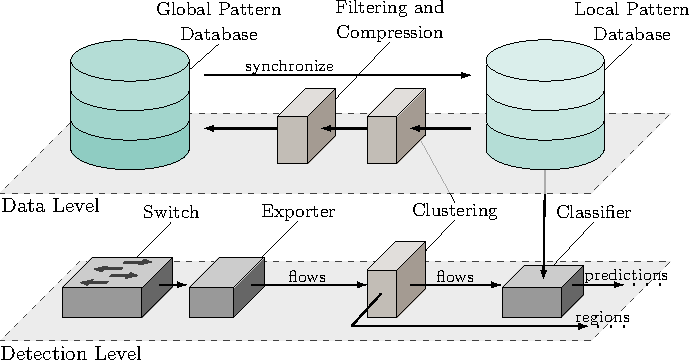
\includegraphics[width=1\linewidth]{tikz/high_level_architecture.pdf}
    \caption{High level CIDS architecture.}
    \label{fig:high_level_architecture}
    \end{figure}

The proposed CIDS exhibits a hierarchical architecture (see Figure \ref{fig:high_level_architecture}). On top, the global infrastructure $G$ provides services, that are globally available to a number of $M \in \mathbb{N}$ local infrastructures $L_m, m \in \{1, \dots, M\}$ that represent the corresponding IT infrastructure boundaries of participating CIDS members. Each $L_m$ agrees to a specified feature extraction process that provides the monitoring data $\bm{X} \subset \mathbb{R}^d$ for attack detection, where specific instances are referred to as $\bm{x} \in \bm{X}$ of size $d = |\bm{x}| \in \mathbb{N}$. In addition, the set of targets $Y \subset \mathbb{N}$ with instances $y \in Y$ is known and registered within each $L_m$. Within every $L_m$, an individual training dataset $D_m= \{(\bm{x}_n, y_n): 1 \leq n \leq N_m\}$ of size $N_m = |D_m| \in \mathbb{N}$ is provided. CIDS communication across local boundaries occurs exclusively in a vertical direction. Thus, the exchange of information between individual $L_m$ takes place indirectly via the global pattern database $(PDB_G)$ and the global event channel $(C_G)$. Each $L_m$ includes a local pattern database $(PDB_{L_m})$, a local event channel $(C_{L_m})$ and an event-based data processing pipeline that consists of four services.



\subsection{Pattern Database} \label{subsec:pattern_database}
Each instance of a pattern database $(PDB)$ is realized as a key-value store. For the following algorithm descriptions, a $PDB$ is treated as a hash table as defined in Section \ref{subsec:hash_table}, referred to by replacing the function variable with the service identifier, e.g. $PDB_G(k)$ being a specific slot or hash value related to a key $k$ in the global pattern database. Note that if a specific hash function is already used to construct a key (e.g. Random Projection), the hash table will internally apply a distinct hash function on the key to ensure even distribution across the slots. 

\subsection{Event Channel} \label{subsec:event_channel}
Event channels provide a topic-based publish-subscribe messaging mechanism that is mainly used to distribute workloads among the service instances in the processing pipeline. Via the messaging system, service instances receive and emit events, on which upon the respective operations are triggered. Changes in a pattern database result in responses that in turn are leveraged as the respective events. In this fashion, updates are propagated throughout the processing pipeline, ensuring a timely consistency among the pattern databases.

\subsection{Processing Pipeline} \label{subsec:processing_pipeline} 
Local and global pattern databases serve exclusively as data sources and sinks for operations. The only exception is the initial import of datasets $D_m$ into the \textit{Local Indexing} service via the messaging system.



\section{Local Indexing}

\begin{figure}[b]
    \centering
    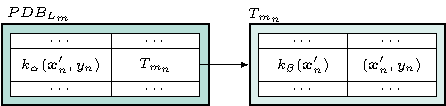
\includegraphics[width=1\linewidth]{tikz/indexing.pdf}
    \caption{Nested indexing in a local pattern database.}
    \label{fig:indexing}
\end{figure}

The local indexing service listens on $C_{L_m}$ for new data points from $D_m$. First, data points are buffered until a defined batch size is released. Subsequently, the batch $X$ is scaled to the range $[-1, 1]$ by applying a feature-wise min-max normalization, given by

\begin{align*}
    \bm{X}' = \frac{\bm{X}-min(\bm{X})}{max(\bm{X}) - min(\bm{X})} \cdot (b - a) + a, \quad
    \setlength\arraycolsep{2pt}
    \begin{array}{lr}
        a = &-1 \\
        b = & 1    
    \end{array}.
\end{align*}

After that, each element $\bm{x}' \in \bm{X}'$ is subject to both a \textit{GRP} $h$ with a global seed for the initialization of the projection plane $\bm{M}$ (see Section \ref{subsec:gaussian_random_projection}) and a non-cryptographic hashing function $g$ (see Section \ref{subsubsec:non-cryptographic-hashes}). The \textit{GRP} clusters the data by mapping similar data points $\bm{x}'$ to the same hash value. The non-cryptographic hashing function on the other hand serves as a mechanism for deduplicating identical $\bm{x}'$. In order to insert a pair $(\bm{x}'_n, y_n) \in D_m$ into the $PDB_{L_m}$, at first two keys $k_\alpha, k_\beta \in K$ are constructed as

\begin{align*}
    k_\alpha(\bm{x}'_n, y_n) &= p_x \doubleplus h(\bm{x}'_n) \doubleplus y_n,\\
    k_\beta(\bm{x}'_n) &= g(\bm{x}'_n),
\end{align*}

where $\doubleplus$ indicates the concatenation operator and $p_x$ describes an arbitrary prefix constant. Secondly, if not already present, a hash table $T_{m_n}$ is created and inserted into the slot $PDB_{L_m}(k_\alpha(\bm{x}'_n, y_n))$. Finally, $(\bm{x}'_n, y_n)$ is hashed into the slot $T_{m_n}(k_\beta(\bm{x}'_n))$. That nested indexing is depicted in Figure \ref{fig:indexing}. Since a particular $h(\bm{x}')$ is a cluster of similar data points, we refer to it as a \textit{region}. Therefore, every region is represented by one or more hash tables $T_{m_n}$, each of them containing data points that belong to the same label. Each execution of that insert operation is executed idempotently, such that the pattern database only returns a response upon the insertion of new data points. For each response, the corresponding region $h(\bm{x}'_n)$ is sent into the local event channel $C_{L_m}$ as an event that indicates a change on a certain cluster within the local pattern database.

\section{Complexity Estimation}

A region is said to be complex, if it contains more than one unique label. Otherwise, a region is simple. Since the data within a region already represents a cluster, the existence of multiple classes indicates a more complex decision boundary. On that basis we differentiate how a region is processed in the subsequent services of the pipeline. Furthermore, the complexity state of a region may vary, depending on the scope it is observed. Note that since the projection matrix $\bm{M}$ is initialized with the same values in every $L_m$, all hashes that were computed by $h$ are globally comparable. This means that similar data points from different datasets, e.g. $\bm{x}_i \in D_1$ and $\bm{x}_j^* \in D_2$ may be hashed to the same region $h(\bm{x}_i) = h(\bm{x}^*_j)$. However, it is also possible that that the corresponding labels $y_i \in D_1$ and $y^*_j \in D_2$ are not equal and therefore lead to a different global view on that region's complexity state. Given that, the complexity estimation module acts as a bridge between the local and global components and answers the question, which regions are considered to be complex in a global context. First, an event containing a region $h(\bm{x}'_n)$ is received. This event is then used for retrieving the set of unique labels $Y_{h(\bm{x}'_n)}$ for that particular region stored at $PDB_{L_m}$, which is defined as

 \begin{align*}
    \bigcup_{y \in Y} \! \Bigl\{ y_n \! \in \! \bigl\{T_{m_n}\bigl(k_\beta(\bm{x}'_n)\bigl)\bigl\} : \! T_{m_n} \! \! \in \! \bigl\{PDB_{L_m}\bigl(k_\alpha(\bm{x}'_n, y) \bigl)\bigl\}\Bigl\}.
 \end{align*}

 Next, a key $k_\gamma \in K$ is constructed by concatenating an arbitrary prefix constant $p_y$ with the region $h(\bm{x}'_n)$ and the id of the current local infrastructure $m$:

\begin{align*}
    k_\gamma(h(\bm{x}'_n), m) = p_y \doubleplus h(\bm{x}'_n) \doubleplus m.
\end{align*}

 Then, $Y_{h(\bm{x}'_n)}$ is inserted into the global pattern database at the slot $PDB_G(k_\gamma(h(\bm{x}'_n), m))$. The global complexity $c_{h(\bm{x}'_n)} \in \{0, 1\}$ is determined by combining the respective label sets from all local infrastructures and evaluating its cardinality:
 
 \begin{align*}
    c_{h(\bm{x}'_n)} = \Bigl| \bigcup_{m \in M} \Bigl\{ PDB_G\bigl(k_\gamma(h(\bm{x}'_n), m)\bigl) \Bigl\}\Bigl| > 1.
 \end{align*}

 Finally, the state $c_{h(\bm{x}'_n)}$ is inserted in the global pattern database by constructing a key $k_\kappa \in K$ with a prefix constant $p_c$ and the region $h(\bm{x}'_n)$ as

 \begin{align*}
     k_\kappa(h(\bm{x}'_n)) = p_c \doubleplus h(\bm{x}'_n)
 \end{align*}

and storing it in the slot $PDB_G(k_\kappa(h(\bm{x}'_n)))$. If the state has changed, a response is returned and the corresponding region $h(\bm{x}'_n)$ is sent as an event into the global event channel $C_G$.

\section{Generative Fitting}

\section{Classifier Fitting}% ~25 pages

    \chapter{Experimental Evaluation}% ~20 pages

    \chapter{Conclusion and Outlook}

\subsection{Conclusion}

\subsection{Outlook}% ~5 pages


\backmatter

    % \include{appendix.tex}
    \printbibliography%
    % \include{abbreviations.tex}
    % \include{list_of_abbreviations.tex}
    % \include{list_of_tables.tex}


\end{document}